\chapter{Evaluation}
\label{cha:evaluation}

Having in mind our hypothesis: "Is it practical to monitor walkers and their users by sending data over LoRaWAN?"

The parameters of our system that have to be measured to test practicality were outlined in the introduction and the tests we intended to run were outlined in the "Design and Methodology" chapter.


\section{Normal Usage}

	\subsection{Pourpose}
		We are running this big experiment because measuring accuracy, consistency, reliability, latency and energy consumption, all have in common the fact that the best way to get data on these parameters is simply using the walker, so we devised this test, which has the goal of helping us simultaneously assess all the aforementioned quality parameters.

	\subsection{Expectations}
		\subsubsection{Consistency}
			We have different expectations, depending on the sensor:

			\begin{enumerate}
				\item Heart Rate: The sensor we are using is very sensitive to noise and we have no way of keeping our heart rate constant when running the test, so we expect the readings to vary quite a lot.
				\item Movement: Since this is a boolean value, we expect it to be quite consistent, always reporting movement or no movement, given the same scenario.
				\item Pressure: We expect that if we manage to put constant force on the pressure sensors, they will give consistent readings
			\end{enumerate}

		\subsubsection{Accuracy}
			Again, each sensor can be said to be accurate if it meets conditions specific to it 

			\begin{enumerate}
				\item Heart Rate: The sensor we are using is very sensitive to the pressure put on it and the thickness of the person's skin. We are also calculating the user's heart rate by processing the raw pulse data, so we don't expect much accuracy
				\item Movement: We are only using the accelerometer to measure if the walker is moving, so we expect an accuracy of 100\%, since we see no reason it would give an erroneous report
				\item Pressure: The pressure sensor we use does not provide an accuracy threshold, but from our preliminary usage it seems to be at least 95\% accurate
			\end{enumerate}

		\subsection{Reliability}
			The only failure we could see happening in this experiment would be LoRaWAN packets being sent from the node to the gateway being dropped, which doesn't seem to happen very often. We are thus expecting at least 90\% reliability. 

		\subsection{Latency}
			The air-time of LoRaWAN packets is dependent on the payload, the distance to the gateway, the spreading factor and much more, so it is hard for us to make an accurate prediction. We have nonetheless noticed, while building our system, that the time between packets is usually between 4 and 9 minutes, so we are expecting an average of around 6 minutes and a high standard deviation from the mean.
		\newline
		\newline
		\newline
		\subsection{Energy consumption}
			The power consumption of our components is as follows:

			\begin{table}[h]
				\begin{tabular}{@{}ll@{}}
					\toprule
					Sensor         & Max current draw (mA) \\ \midrule
					Pulse          & 4                     \\
					Pressure (x2)  & 3                     \\
					Accelerometer  & 0.5                   \\
					GPS            & 57                    \\
					LoRaWAN shield & 10                    \\
					Mega 2560      & 80                    \\
					Total          & 159                   \\ \bottomrule
				\end{tabular}
				\caption[Energy consumption Arduino]{Energy consumption Arduino}
				\label{tab:EnergyConsumption}
			\end{table}

			Based on this, we expect the current draw to be around 160mA

	\subsection{Parameters}
		We had on of our team's members use the walker normally for 30 minutes, while the information was coming in and stored in our server for analysis. There were only three details:

		\begin{itemize}
		  \item In order to test the accuracy of the heart rate, we had the team member testing the walker use an Iwatch for comparison, which is also not the most accurate of devices, but we don't have access to a better one
		  \item In order to test the consistency of the pressure sensor readings, we put an elastic band applying constant force on the right handle's sensor
		  \item In order to measure the current draw we used a USB Current Meter during the experiment
		\end{itemize}

	\subsection{Results}
		
		\subsubsection{Heart Rate}
			First run:
			\begin{figure}[h]
				\centering
				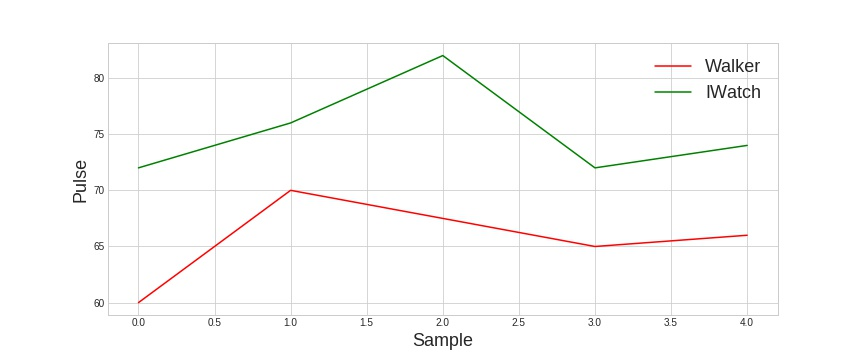
\includegraphics[width=1.1\linewidth]{gfx/pulse_run1_diff.jpg}
				\caption{Measurement heart rate first run}
				\label{fig:HeartRateFirst}
			\end{figure}
			
			Second Run:
			\begin{figure}[h]
				\centering
				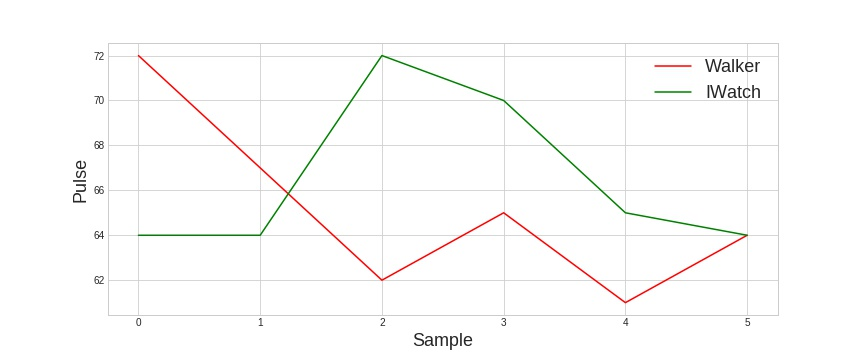
\includegraphics[width=1.1\linewidth]{gfx/pulse_run2_diff.jpg}
				\caption{Measurement heart rate first run}
				\label{fig:HeartRateSecond}
			\end{figure}

		\subsubsection{Reliability}
			All the packets arrived successfully, but in two of them the heart rate was 0.

		\subsubsection{Latency}
			Here are the times, in minutes and seconds, between packets:
			\begin{table}[h]
				\begin{tabular}{@{}lll@{}}
					\toprule
					\textbf{Gap}&\textbf{First Run}& \textbf{Second run} 	 \\ \midrule
					1st - 2nd 			&	7:35		& 	6:00     	 \\
					2nd - 3rd 			&	8:06    	& 	4:43         \\
					3rd - 4th 			&	6:47		& 	5:05         \\
					4th - 5th 			&	6:13    	& 	5:14         \\
					5th - 6th 			&	         	& 	4:24         \\ \bottomrule
					average     		&   7:18        &   5:05		 \\
					Standard deviation  &   50.13s      &   36.30s		 \\ \bottomrule
				\end{tabular}
				\caption[LoRaWAN latency]{LoRaWAN latency}
				\label{tab:Latency}
			\end{table}
		
			\begin{figure}[h]
				\centering
				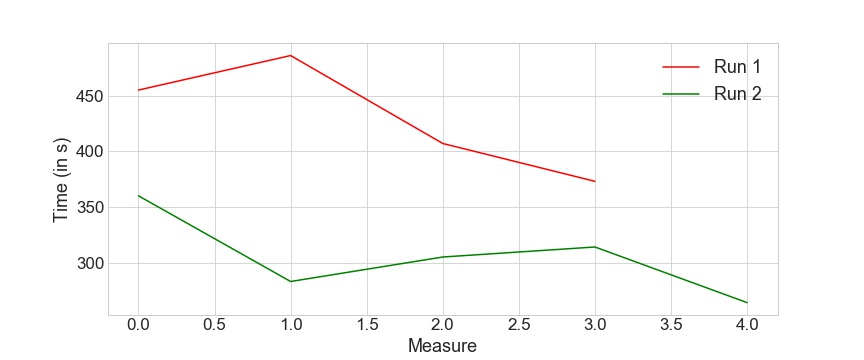
\includegraphics[width=1.1\linewidth]{gfx/latency_diff.jpg}
				\caption{LoRaWAN latency}
				\label{fig:Latency}
			\end{figure}

			Int the 1st run we got an average of 7:18, with a relative standard deviation of 11.7\%, while in the second run we got an average of 5:05, with a relative standard deviation of 11.9\%.

		\subsubsection{Energy consumption}
			The walker used 105 and 104 mAh during the first and second runs respectively. This means it was drawing a current of around 210mAh

	\subsection{Matching results and expectations}
		\subsubsection{Heart Rate}
			In both runs we got a reading of 0 in on of the measurements, so we will takes these as errors of the overall system and not take them into account in our statistical analysis.

			In the first run we got a mean average percentage error (MAPE) of 11.27, between this and the second run, we found an improvement that could be done to the algorithm, so we changed it for the second run, where we got a MAPE of 7.94. Given the constraints mentioned in our expectations, these results are better than we expected, perhaps because %34r come up with explanation

			We believe doing an analysis of the precision is not appropriate, since there was a gap of several minutes between measurements and the person was walking around, so there is no reason we should expect the heart rate to be constant.

		\subsubsection{Pressure}
			Regarding Accuracy, we had no way to get the real value of the pressure being applied on the handle while the walker is in use, so it doensn't seem like a relevant analysis to do. We have nonetheless previously tested the pressure sensors with a 1kg bag of rice, and both reported that exact value, so we can expect them to be similarly accurate while in use on the walker.

			We got a relative standard deviation of 8.27\% on the first run and 4.76\% on the second one, which is whithin our expectations. The deviations we see could be explained by the movement of the walker itself and/or changes in the position of the elastic band.

		\subsubsection{Movement}
			As expected, we got an accuracy of 100\% on the movement detection, and, since it is a boolean value, also a standard deviation of 0. Getting the movement status of the walker is a very simple measurement, so any result other than this would have been surprising.

		\subsubsection{Reliability}
			We believe the two failed measurements are due to the method we have for calculating the heart rate from the pulse, which times out if it doesn't find a value within a certain time frame, so that is most likely what happened in both these cases. We can notheless say that the whole data pipeline was 100\% reliable, which is the most relevant parameter for our hypothesis.

		\subsubsection{Latency}
			We got, on both runs, equaly spread out times, which is good evidence for the consistently high variablity of the latency, which is what we had expected. Our expectation of 6 minutes average time is right in the middle of the two runs (7:18 and 5:05), which leads us to believe that if we did more and longer runs, it would converge somewhere between 5:30 and 6:30.

		\subsubsection{Energy consumption}
			The walker consumed 30\% more than we expected, we think this could be because we are using two of the 5V pins, but it is most likely a factor we are not aware of and decided investigating it would be out of the scope our knowledge and most importantly this project.

\section{Idle Energy Consumption}

	\subsection{Pourpose}
		Most of the time, the walker will not be in use, so it is important to know how much energy it draws while idle
	\subsection{Expectations}
		When the walker is not moving, the only activity the Arduino does is checking the movement status every 15 seconds. We nonetheless have reason to think that just the fact that the sensors are connected has them draw current, so we expect the power consumption to be close but a bit less than to that of the walker in use, which we expected to be 160mA.
	\subsection{Parameters}
		We connected a USB Current Meter to the walker and left it idle for 12:30h the first time and the 18:00h the second time
	\subsection{Results}
		During the 12:30h window, the walker drew 2498mAh, which equates to an average current of 200mA, while in the 18 hour run it drew 3505mAh, equating around 195mAh.
	\subsection{Matching results and expectations}
		As in the normal usage experiment, the Arduino drew much more current than the expected, and the explanation we have is the same. It was, as we predicted, just a bit lower than that of the walker in use, meaning a future improvement over our system would be setting up the node such that the sensors are not drawing power while the walker is idle.

\section{Integrating the GPS sensor}
	\subsection{Pourpose}
	This experiment has the goal of figuring out how quickly a new sensor can be added to the walker. Our walker is a proof of concept for something bigger, so it is important to know how extensible it is.

	\subsection{Expectations}
	Having in consideration how much time it took us to mount, get readings, and send the current sensor's information, we expect to take around 1 or 2 days to integrate the GPS sensor into the system. 

	\subsection{Parameters}
	For this experiment, we had two of the team's members work exclusively on integrating the GPS sensor into the system. This consisted in mounting it on the walker, getting some readings, figuring out the best way to encode the data for sending over LoRaWAN, and then adapting the rest of the components to handle the latitude and longitude.

	\subsection{Results}
	Integrating GPS into the system ended up taking 2 whole days, not only was it hard to find a port layout which allowed all the sensors to work, but library support is also not very good, so after unsuccessfully trying to use external libraries, we ended up implementing it ourselves, which took some extra time.

	\subsection{Matching results and expectations}
	Integrating GPS into our system took as much time as we were roughly expecting, perhaps it is on the higher end of our expectation because of the usual delays that come with getting the right documentation for sensors and how they interplay with the other components. Two days doesn't seem like much having in consideration that repeating the process on new nodes would be much faster the following times.

	While performing this experiment, coincidentally, we noticed that when the GPS wasn't working and we wanted to use the walker for other tests, we had to remove it, so we could also say the system is modular in the sense that it is easy to remove sensors.

\section{Testing the GPS sensor}

	\subsection{Pourpose}
		This experiment will allow us to know the accuracy and precision of the GPS sensor
	\subsection{Expectations}
		According to the specification, the NEO 6M module should be accurate within 2 meters, so that is our expectation. Regarding precision, our module's datasheet does not provide a threshold, so we don't know what to expect there,

	\subsection{Parameters}
		We took the walker outside and got its location through the GPS sensor 40 times

	\subsection{Results}
		The GPS had an average error of 3.5 meters, and the following error distribution:

		\begin{figure}[h]
			\centering
			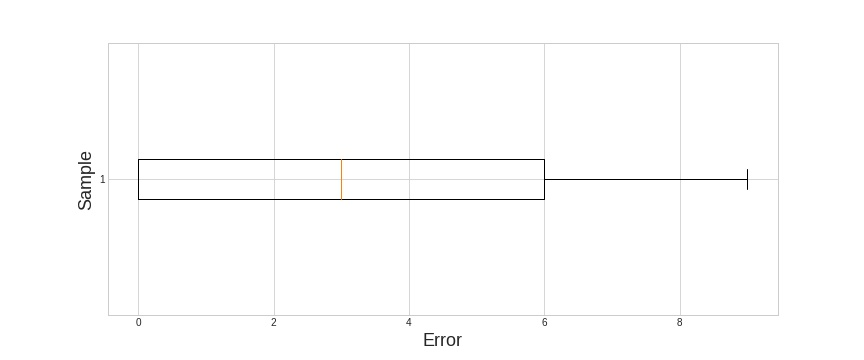
\includegraphics[width=1.2\linewidth]{gfx/gps_boxplot_error}
			\caption{GPS error boxplot}
			\label{fig:GPS plot}
		\end{figure}

	\subsection{Matching results and expectations}
		The GPS was less accurate then expected, perhaps because of being positioned in the side of the walker, not getting the perfect reception.


\section{Setting up the Arduino from scratch}

	\subsection{Pourpose}
		With this experiment we can get an idea of how scalable our system is, which is one of its most important features.
	\subsection{Expectations}
		We expect the first atempt to take around 4 minutes because we haven't registered a device in a while, but if the process is streamlined we expect it to take around 1:30 minutes, since it just requires navigating menues and slighly changing the node.
	\subsection{Parameters}
		We will, on the same computer, register a new device in The Things Network, change the node files to include its new authentication codes and upload them to the Arduino.
	\subsection{Results}
		The first atempt took 4:50 and the second one 01:02.
	\subsection{Matching results and expectations}
		The first atempt took a bit longer than expected, perhaps because we didn't remember very well how to navigate the menus and options on The Things Network. On the second run we were even faster than predicted, maybe because what takes the most time is simply navigating the menus, and after knowing exacly what do it is very fast. This experiment is not a complete demonstration of the scalability of our system, but it is the best we could come up with given the resources. It doesn't show how the system would handle several nodes in parallel but at least we know that the act of adding them would be quick.

\subsection{Disconnecting cables}

	\subsection{Pourpose}
		We wanted to have a test for accessing the serviceability of the walker, this will allow us to have an idea of how long the walker will take to be fixed when hardware problems arise.
	\subsection{Expectations}
		We expect the node to be fixed in around 2:30 minutes, which includes looking up the supposed layout and arranging the cables accordingly.
	\subsection{Parameters}
		One of the team members will disconnect 7 random cables from the node and another one will atempt to fix it.
	\subsection{Results}
		The node was back up and running in 1:22, having the first packet arriving on our server at 1:28.
	\subsection{Matching results and expectations}
		We overestimated the time it would take by a minute, we think this might be because the team member fixing the walker was the most familiar with the cabling and pin layout.

\section{Finding maximum throughput}

	\subsection{Pourpose}
		We dont intend to send much information, but it is nonetheless usefull knowing how much could theoretically be sent
	\subsection{Expectations}
		We have configured our system to be able to use a spreading factor between 7 and 12, which have a maximum payload of 222 and 51 bytes, respectively, so we are expecting any value in-between, but most likely one of these two, since they are the most commonly used.
	\subsection{Parameters}
		We will increase the payload by 
	\subsection{Results}
		We kept increasing, testing twice and decreasing the payload in the following fashion, until we found the maximum we could successfully send:

		\begin{table}[h]
			\begin{tabular}{@{}lllllllllll@{}}
				Payload (bytes) & 15  & 30  & 60 & 45  & 50  & 55 & 54 & 53 & 52 & 51  \\
				Success & yes & yes & no & yes & yes & no & no & no & no & yes
			\end{tabular}
			\caption[Payload testing LoraWAN]{Payload testing LoraWAN}
			\label{tab:LoraWanPayload}
		\end{table}

		For the payloads of 60, 55 and 54 bytes, the packets never arrived at ttn, for loads of 53 and 52 bytes, they arrived but the payload was not readable.

	\subsection{Matching results and expectations}
		The maximum payload we got was 51 bytes, which is one of the options we considered most likely. With this experiment we can be sure the system is using a spreading factor of 12, which provides a very long range, but a very small payload and thus small throughput.

%%% Local Variables:
%%% mode: latex
%%% TeX-master: "../ClassicThesis"
%%% ispell-dictionary: "british" ***
%%% mode:flyspell ***
%%% mode:auto-fill ***
%%% fill-column: 76 ***
%%% End:
